%\documentclass[reprint,pra,twocolumn,superscriptaddress]l{revtex4-2}
%[aps,prl,singlecolumn,superscriptaddress]
\documentclass{article}
\usepackage[english]{babel}
% \usepackage{ucs}
% \usepackage[utf8x]{inputenc}
\usepackage{amsmath}
\usepackage{amsfonts}
\usepackage{amssymb}
\usepackage{graphicx}
%\usepackage{bm}
\usepackage{bbm}
\usepackage{empheq}
\usepackage{color}
%\usepackage{pdfpages}

%\usepackage{graphicx}
%\usepackage{color}
%\usepackage[dvipsnames]{xcolor}
%
%\usepackage{a4wide}
\usepackage[backend=bibtex]{biblatex}
% \bibliographystyle{apsrev_lyy}
\bibliography{SiGe_ref_v1}


\begin{document}
	
\title{Radio frequency reflectometry for qubit readout in silicon based quantum dot}

\author{Y.-Y. Liu}
\author{S. G. J. Philips}
\author{L. A. Orona}
\author{N. Samkharadze}
\author{L. M. K. Vandersypen}
\author{A. Yacoby}

\date{\today}


\begin{abstract}
RF reflectometry for charge sensing is a fast and high fidelity method for spin qubit measurements.  While it has been successfully implemented in gallium arsenide, silicon germanium has proved significantly more challenging due to substantially larger capacitances of the devices to ground.  We demonstrate that the effects of this extra capacitance can be mitigated to enable RF reflectometry.  Additionally, we demonstrate that this capacitance can actually serve as a pathway to introduce the RF tone to the sensor dot.  We lay out the considerations for these two techniques.
\end{abstract}

\maketitle

\section{Intro} % (fold)
	\label{sec:intro}
	As Moore’s law begins to break down, new computational schemes will be necessary for improved computation performance.  Quantum computing is an exciting avenue that already boast algorithms that should provide speedups or perform tasks that are impossible on conventional computers (\textcolor{red}{cite papers on quantum computation algorithm/proposals}).  Of the physical platforms available, spin based quantum bits (qubits) in semiconductors are particularly promising \cite{Morton11} \textcolor{red}{cite papers on GaAs/SiGe/InAs/... spin qubit}).  These qubits can be initialized quickly and with high fidelity through spin dependent tunneling to a neighboring Fermi sea.  Single qubit gates with fidelities above 99\% and two qubit gates above 90\% have been demonstrated.  The small size and localized nature of the control also lend themselves naturally to scaling to the number of qubits needed for a fully functioning quantum computer. One particularly interesting semiconductor material is silicon germanium (SiGe) which hosts a two dimentional electron gas (2DEG) where spin qubits can be formed. The qubit overlaps with orders of magnitude less nuclear spins than in other materials, such as gallium aresenide (GaAs), which reduces decoherence due to the magnetic field noise from nuclear spin fluctuations \textcolor{red}{cite papers}. 

	Charge sensing is an important technique for measuring spin qubits because their long-lived spin states can be converted into detectable charge states.  This is usually done by Elzerman readout or Pauli-Spin blockade readout (\textcolor{red}{papers}). To detect a charge state, one can make use of a sensing quantum dot (SD) in close proximity (d $< \sim$  300 nm) to the qubit. The current through the sensing dot is strongly dependent on the charge state of the qubit because the electric potential of the qubit shifts the Coloumb peaks of the sensor dot, drastically altering its resistance. 	The easiest (and most commonly used) way to measure this is by using a DC current through the sensing dot with a amplifier at room temperature (e.g. with a JFET). However, this requires an integration time on the order of milliseconds, drastically slowing experiments because intializing and manipulating the qubit can be done on the nanosecond or microsecond scale.  To reduce the noise, people have also built low temperature DC amplifiers that are operated within the same dilution refrigerator as the qubit.  This is technically difficult \textcolor{red}{Mark's paper?} due to issues like heating.  For this reason, high frequency techniques that allow for filtering of low frequent noise and several microsecond integration times are of great interest. 
	
	Radio Frequency (RF) reflectometry was originally proven to be a very effective technique in GaAs spin qubits and has enabled single shot readout with only several microseconds of integration \cite{Schoelkopf1998} \textcolor{red}{more papers?}. However, SiGe has proved to be a more challenging platform in which to implement RF reflectometry due to larger capacitances to ground. Typical GaAs substrates are depletion mode while SiGe wafers are most often grown undoped so that they are accumulation mode and require metallic electrostatic gates to cover all current paths so that the 2DEG can be populated \textcolor{red}{design papers?}. This capacitive coupling between the 2DEG and gates is undesirable for RF reflectometry because it provides low impedance leakage pathways to ground that are independent of the SD. This reduces the sensitivity of the reflected signal to the qubit state. Previous work has addressed this problem by the use of resistors \cite{Volk2019} and careful design of the accumulation gates \cite{Connors2020}.  In this work, we further develop the understanding of the leakage pathway introduced by this capacitance and introduce a new method for achieving reflectometry.
	
	Here we demonstrate that RF reflectometry can be achieved in SiGe using two general approaches that differ in how the measured RF signal is carried to the lead of the SD.  In the ohmic style, the signal enters the 2DEG through an ohmic contact so that it carried in the 2DEG itself all the way to the SD, as in GaAs.  For this approach, it is important to mitigate the effects of capacitance as much as possible.  In the split gate style, the RF signal is carried by a gate which is capacitively coupled to the lead in the 2DEG near the sensor dot.  For this approach, the capacitance is a resource and not a detractor because the capacitance is what enables the signal to reach the SD.  For both schemes, we have achieved sensitivity of the RF reflection to the resistance through the SD and have performed charge readout of the target quantum dot.  
	
\section{RF Reflectometry}
	\label{sec:rf_reflectometry}


	\begin{figure}[h]
		\includegraphics[width = \columnwidth]{figures/overview3.pdf}
		\caption{(a) Sample mounted and wired bonded to a circuit board.  False color image of scanning electron micrograph of a typical SiGe overlap style device.  (b) Sketch of the gate layout for the ohmic approach where the signal is applied to the SD through the ohmic.  (c) Continuous model circuit diagram for the ohmic method.  The bracketed section represents that the device has distributed capacitance and resistance.  (d) Lumped element circuit diagram for the ohmic method.  The distributed capacitance and resistance are replaced with lumped elements for computational simplicity. (e) Circuit diagram and sketch of the gate layout for the gate approach where the signal is applied to the SD through the accumulation gate. }
		\label{fig:overview}
	\end{figure}


	\label{sub:why_sige_is_very_different_from_the_simples_reflectometry}
	In RF reflectometry a fixed frequency signal is reflected off an impedance matching inductive capacitive (LC) tank circuit that is loaded with the SD with resistance $R_{\rm SD}$, as shown in Fig.\ \ref{fig:overview}(c). The reflection coefficient of this tank circuit is given by $\Gamma=(Z-Z_0)/(Z+Z_0)$, where $Z$ is the impedance of the loaded tank circuit and $Z_0 = 50 \Omega$ is the source impedance. When the device's parasite capacitance $C_{\rm 2DEG}$ and contact resistance $R_{\rm 2DEG}$ can be ignored, the effective impedance of the loaded tank circuit is $Z = i2\pi fL + 1/(1/(R_S + i2\pi fC_0)$ at an input frequency $f$. In the experimental setup $L$ is a lumped element inductor and $C_0$ represents the total capacitance to ground of the circuit board, a lumped element capacitor and the parasitic capacitance of the bond wires of the device. 

	$\Gamma$ is strongly modulated near $\Gamma = 0$, which occurs at the matching condition that $Z=Z_0$ when driven with $f$ equal to the resonant frequency of $f_M=1/(2\pi \sqrt{LC_0})$ and with $R_{SD}$ equal to the matching resistance $R_M=L/C_0Z_0$. $R_{SD}$ is very sensitive to the electric potential of the SD's environment, and thus to the charge states in the nearby quantum dots used to form the qubits.  Hence $\Gamma$ is sensitive to the charge state of the qubit because of its dependence on $R_{SD}$.  The tank circuit is designed with $L$ and $C_0$ chosen so that the value of $R_M$ is where $R_{SD}$ is most sensitive to the qubit, typically in the range  of 50 -- 600 $k\Omega$.  For GaAs, this simple model is sufficient to capture the observed behavior. 


	In SiGe, the simple tank circuit model fails because $R_{\rm 2DEG}$ and $C_{\rm 2DEG}$ are no longer negligible.	Figure\ \ref{fig:overview}(a) demonstrates a typical overlap style device.  A quadruple quantum dot is formed with the lower set of gates and two sensors are formed with upper gates. Large accumulation gates control the electron density of the leads from the ohmic contacts to the quadruple dots used to form the qubits and the SDs.  Compared to depletion mode devices, there is an additional $C_{\rm 2DEG}$ of 0.1--1 pF because of the accumulation gate, as seen in Figure\ \ref{fig:overview}(b).  The RF signal used for reflectometry passes through the lossy 2DEG channel with resistance $R_{\rm 2DEG}$ and is shunted to ground through $C_{\rm 2DEG}$, drastically reducing the sensitivity of $\Gamma$ to $R_{SD}$ so that the qubit charge state cannot be detected. 


	To overcome this problem, we demonstrate two alternate approaches:
	\begin{itemize}
		\item Ohmic Approach -- Couple the tank circuit to the ohmic but mitigate the effects of $C_{\rm 2DEG}$ and $R_{\rm 2DEG}$ through engineering of the circuit board that carries the sample and elements used in the tank circuit, Figure\ \ref{fig:overview}(b).
		\item Split Gate Approach -- Couple the tank circuit to the accumulation gate so that the signal capacitively enters the lead of the SD, Figure\ \ref{fig:overview}(e).  This means that the signal passes through $C_{\rm 2DEG}$ intentionally and that it is not a leakage pathway.
	\end{itemize}

\section{Ohmic Approach} % (fold)


	\begin{figure*}
		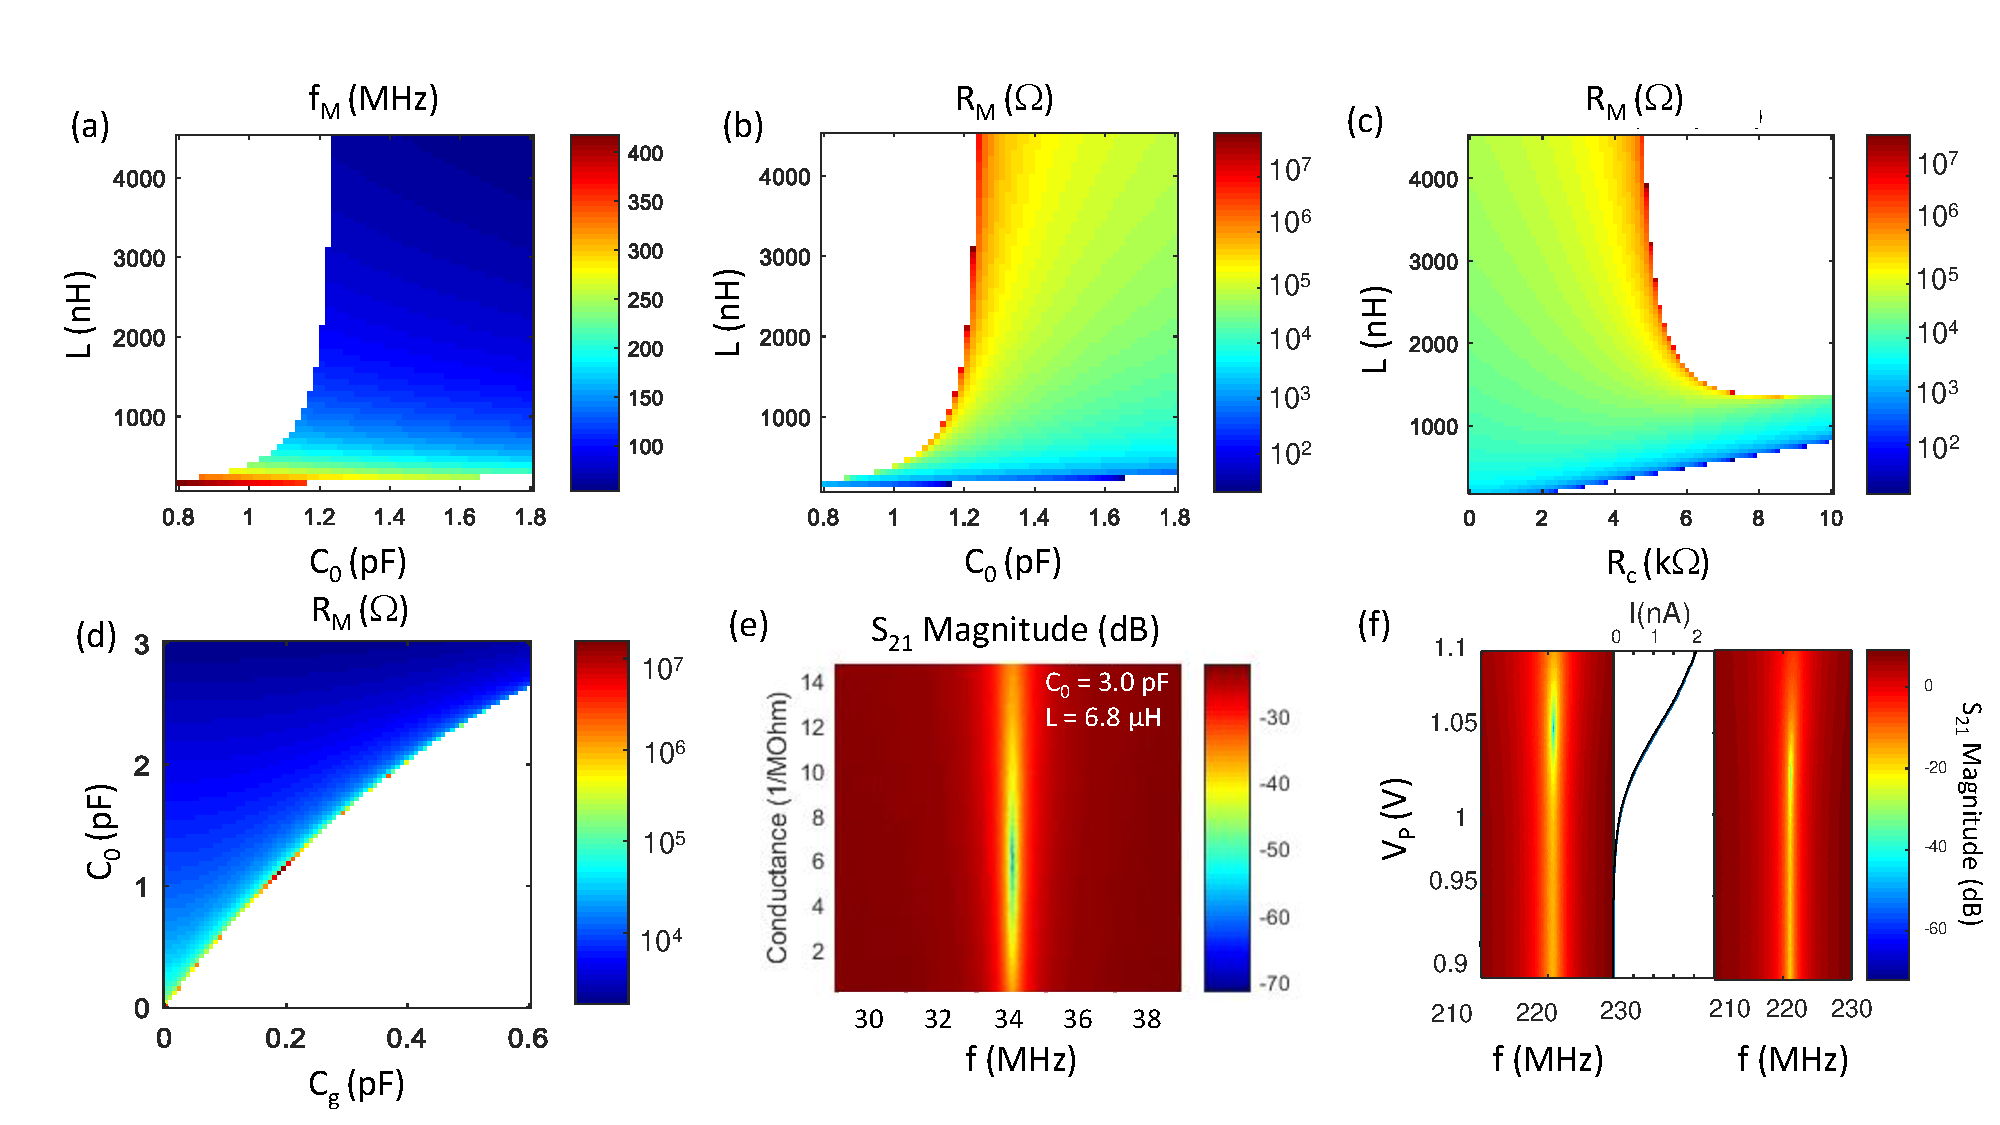
\includegraphics[width = \textwidth]{figures/HarvardFigure2_v7.pdf}		
		\caption{(a) and (b) Simulations of $f_M$ and $R_M$ as a function of $C_0$ and $L$ with fixed parameters of $C^*_g$ = 0.2 pF and $R_c$ = 3 k$\Omega$. White regions are where no matching can be achieved.  (c) Simulation of $R_M$ as a function of $R_c$ and $L$ with fixed $C^*_g$ = 0.2 pF, and $C_0$ = 1.6 pF. (d) Simulation of $R_M$ as a function of $C_0$ and $C^*_g$ with $L$ = 1000 nH, and $R_c$ = 3  k$\Omega$.  (e) Experimental demonstration of best matching with $f_M$ = 34 MHz.  (f) Experimental demonstration of $R_M$ dependence on $R_c$.  While $R_c$ cannot be measured because it is so much smaller than $R_{SD}$, it is dependent on $V_L$.  The left panel has $V_L$=1 V and the right panel has $V_L$=0.45 V and have $R_M$=67 k$\Omega$ and $R_M$=200 k$\Omega$ respectively.
		}
		\label{fig:Harvard}
	\end{figure*}



		\label{sub:ohmic_approach_circuit_and_model}
		
		The ohmic approach is shown in Figure\ \ref{fig:overview}(b) and introduces the RF signal to the lead of the SD through the ohmic contact, as in  GaAs.  The significant resistance of the 2DEG and capacitance to the accumulation gate prevent applying the simply RLC model to SiGe devices.  Instead, the device has distributed capacitance and resistance, as modeled by the series of capacitors and resistors, shown in Figure\ \ref{fig:overview}(c).  For simplicity, this can be treated as a single resistance, $R_c$ and single capacitance, $C_g$, as shown in Figure\ \ref{fig:overview}(d).  We will begin by exploring how the tank circuit parameters ($C_0$ and $L$) and the device parameters ($R_c$ and $C_g$) affect the matching conditions ($f_M$ and $R_M$).  This understanding will then be applied to demonstrate several key strategies that allow for ohmic style RF reflectometry in SiGe.  We must design the tank circuit so that $R_M$ and $f_M$ are experimentally achievable and so that majority of the power is dissipated in $R_{SD}$ to achieve a usable signal to noise ratio (SNR).

	\subsection{Lumped Element Model}

	For the standard tank circuit model, there will always be some $f_M$ and $R_M$ where matching is achieved.  However, simulations and experiments demonstrate that large values of $R_c$ and $C_g$ can prevent there being a $R_M$ and $f_M$ and therefore the ability to use the tank circuit for charge detection.  In Figure\ \ref{fig:Harvard} we explore the dependence of the matching conditions on $C_0$, L, $C_g$ and $R_c$.  Simulations are performed by solving for $R_{\rm SD}$ and $f$ such that the $Z$ of the loaded tank circuit is set equal to $Z_0$ = 50 $\Omega$ to find the values of $R_M$ and $f_M$ respectively.  The constraints that $f_M$ is real and that $R_M$ is real and positive result in there being conditions where no matching can be achieved, which are shown as white regions in Figure\ \ref{fig:Harvard}(a-d).

	When a sample is fabricated, $C_g$ and $R_c$ are roughly fixed, meaning that the only way to change $R_M$ and $f_M$ is through the tank circuit parameters $L$ and $C_0$.  We present numerical simulations of $f_M$ in Figure\ \ref{fig:Harvard}(a) and $R_M$ in Figure \ \ref{fig:Harvard}(b) as a function of $L$ and $C_0$ with $C^*_g$ = 0.2 pF and $R_c$ = 3 k$\Omega$.    We note that far from the non-matching regions, the behavior is approximately that of the standard tank circuit model.  Under these conditions, $C_0\gg C_g$ which means that $C_0$ dominates the capacitance of the loaded tank circuit.  When $C_0$ is comparable to or smaller than $C_g$, there is very little dependence on $R_{SD}$ because the parallel pathway through $C_g$ is low impedance.  

	Achieving best matching with both $R_M$ and $f_M$ in the desired range requires designing the sample with $R_c$ and $C_g$ in mind.  The dependence of the matching conditions is strongly dependent on $R_c$, as shown in Figure\ \ref{fig:Harvard}(c).  At $R_c=0$, the model is reduced to the standard tank circuit model with an effective $C_0^*=C_0+C_g$.  We note that the range of parameters that can achieve matching is drastically reduced as $R_c$ increases.  Reducing the resistance of the lead is therefore key to achieving RF reflectometry.  To understand the impact of $C_g$, we present a simulation the dependence of $R_M$ in Figure\ \ref{fig:Harvard}(d).  We again observe that matching is only achieved when $C_0>C_g$.

	Together, these simulations suggest that the tank circuit itself should provide the dominant contributions to the capacitance through $C_0$ and that all contributions from the device other than $R_{SD}$ should be minimized.  We apply this understanding experimentally in the next section

\subsection{Implementing Ohmic Style RF Reflectometry}

	We have identified several experimental strategies for device and circuit design that enable RF reflectometry in SiGe by using the information provided in the previous section.  

	\textit{Block shunting to ground through $C_g$.}  Simulations have demonstrated that the RF signal in the lead has a low impedance path to RF ground through $C_g$.  The gates themselves are connected to DC supplies and have RC filters to remove noise whose capacitors shunt the RF reflectometry signal to ground.  In order to block this pathway, we have designed our printed circuit board (PCB) to have resistors, $R_b$ between the sample bond pads and the RC filters to increase the impedance of the pathway to ground through $C_g$,  figure \ref{fig:overview}(d).  We use 10 k$\Omega$ 0201 resistors.    

	There is a parasitic capacitance, $C_p$, to ground from all the metal on the sample side of $R_b$ (gate, bond wire, bond pad, PCB trace).  This is in parallel to $R_b$ and limits the ability to decrease the impact of $C_g$ by just increasing $R_b$.  Placing the $R_b$ as close the bond pads as possible is ideal because it minimizes the amount of metal that contributes to $C_p$.  This parasitic capacitance that cannot be entirely removed but it can be reduced by reducing the ground plane near the bond pads and by placing $R_b$ as close to the bond pad as possible.   Our PCB has $R_b$ placed 3 mm away from the bond pads to minimize $C_p$ while still allowing for sample bonding.  Controlling both $R_b$ and $C_p$ serves to decrease the effective $C_g$ that the device sees.

	\textit{Ensure and control matching with $C_0$ and $L$.}  The previous simulations demonstrated that the matching condition can be tuned when $C_0 \gg C_g$.  Our PCB has been designed with solder pads for a surface mount inductor, $L$, and a surface mount capacitor to control $C_0$.  While the inductance of the PCB will be negligible without the surface mount component, the parasitic capacitance (which is not the same as $C_p$ above) will be quite significant, usually on the order of 0.1 to 1 pF.  As much ground plane near the tank circuit should be removed as possible in the design so that that the parasitic capacitance is reduced.  It is always possible to increase $C_0$ through the surface mount element but it cannot be reduced below the parasitic capacitance of the board and for some devices we have found it optimal to have $C_0<$ 1 pF.  

	We have two parameters that we would like to optimize, $f_M$ and $R_M$, using the two design parameters, $L$ and $C_0$.  As previously noted, $C_0$ is has a lower limit set by the parasitic capacitance of the board.  Practically, we need $C_0$ is set as low as allowed by $C_g$ because we want $f_M$ to be larger than 100 MHz.  $L$ has then been chosen so that $R_M$=50-200 k$\Omega$.  We have found success using approximately $L$ = 760 nH and $C_0$ = 0.8 pF.  While tuning $C_0$ and $L$ does enable the tank circuit to achieve matching with a usable $R_M$, it may come at the cost of an unworkably low $f_M$, as in Figure\ \ref{fig:Harvard}(e).  For this reason, it is important to reduce the impacts of $C_g$ and $R_c$.

	\textit{Balancing the impacts of $C_g$ and $R_c$ in sample design.}  The sample design impacts both $C_g$ and $R_c$, both of which we want to minimize, through the length $l$ and width $w$ of the accumulation gate.  Knowing that $C_g\propto lw$ and $R_c\propto l/w$ reveals that decreasing $l$ is ideal for both parameters while decreasing $w$ to improve $C_g$ comes at the cost of increasing $R_c$ and vice versa.  We have found that $w=$5 $\mu$m is sufficient to achieve consistent accumulation for usable $R_c$ without increasing $C_g$ drastically.  The ohmic should be placed as close to the SD as possible to limit $l$ and we have found that a distance of 10 $\mu$m does not decrease device performance.  

	\textit{Tuning $R_c$.}  To experimentally confirm the dependence of $R_M$ on $R_c$, we make use of the lead gate seen in Figure\ \ref{fig:overview}(b).  This gate has a large width so that $R_c$ on the order of 1--10 k$\Omega$ can be achieved.  It is also designed to have a short length and only bridges between the ohmic and the accumulation gate so that it has a small area.  The voltage on this gate can be tuned to vary $R_c$ while minimally effecting $C_g$ because of its small area.  

	In Figure\ \ref{fig:Harvard}(f) we demonstrate a tuneable best matching $R_M$ around 50$\sim~$200 k$\Omega$ at a resonant frequency of 220 MHz. The outside two panels plots the reflection power as a function of voltage applied to the sensor dot plunger gate $V_{P}$ at a higher (left panel) and lower (right panel) voltages applied to the lead gate. The middle panel plots corresponding the conductance of the sensor dot. With different gate voltage on the lead gate, the total conductance through the dot is unchanged with the same voltages of all other gates, indicating a small back-action to the sensor tuning. In the contrast, the best matching is achieved with 67 k$\Omega$ for the fully accumulated switch gate, and 200 k$\Omega$ for a partial accumulated switch gate. The only difference between them is $R_c$ and this result agrees with the simulation in figure\ \ref{fig:Harvard} (c). This tunability allows the use of fixed $C_0$ and L for general devices as the matching condition of the device can be changed in situ.  The tunable $R_c$, however, is not the final solution because the larger $R_c$, more energy is lost before the sensor dot, resulting in a smaller signal.

\section{Split Gate Approach} % (fold)
	%%%%%%%%%%%%%%%%%%%%%%%%%%%%%%%%%%%%%%%%%%
	%% TODO									%%
	%%	* fix color map to jet				%%
	%%	* add figure C2deg vs Rmax/Fres 	%%
	%%	* add bandwidth fig 				%%
	%% How will this impact your sensing scheme? --> answer Yinyu -- no effect, just SNR*2.
	%% Some formula link the SNR and fidelity? --> it seems pretty linear :-p, but the range is to small to fit 
	%% Panel C: can you invert the y axis? 1- or flip?
	%%%%%%%%%%%%%%%%%%%%%%%%%%%%%%%%%%%%%%%%%%

	\label{sub:lead_gate_approach}

	\begin{figure}
		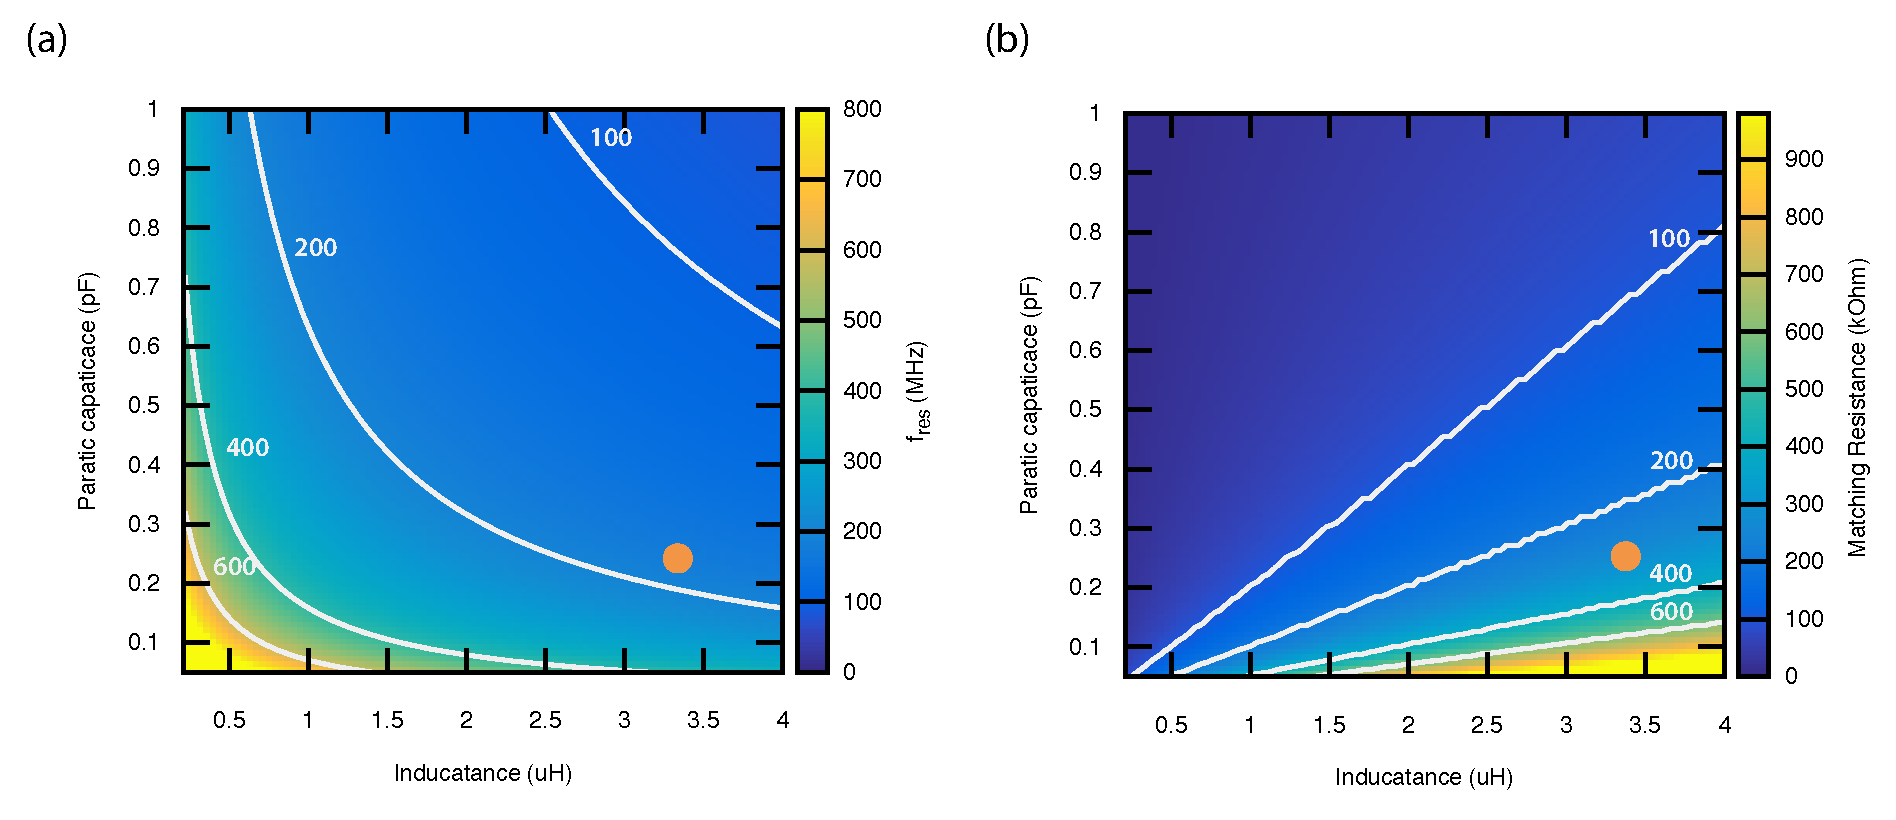
\includegraphics[width=\linewidth]{figures/Theory_figure/theory_delft_v3.pdf}
		\caption{Circuit simulations for the circuit shown in \ref{fig:overview}(c), where the inductance L and the parasitic capacitance $C_p$ are varied. The resistance of the lead gate ($R_{lead}$) is set to 10 M$\Omega$ (typical value used in the experiment), the capacitance of the accumulation gate to the 2DEG is set to 100 fF. The orange dot indicates the parameters for the device and circuit used in this paper.}
		\label{fig:lead_gate_theory}
	\end{figure}

	In this approach, the RF signal is provided via the accumulation gate\cite{Volk2019} instead of the ohmic contact. The capacitive coupling of the accumulation gate to the 2DEG ($C_{2DEG}$) is used to couple the RF signal into the 2DEG. To ensure that the signal does not 'leak' via the ohmic, we  split the accumulation gate into two parts (figure \ref{fig:overview}(e)).
	The gate labeled ‘accumulation gate’ serves to accumulate the 2DEG used as the source reservoir for the sensing dot and the ‘lead gate’ accumulates a second 2DEG, connecting the reservoir 2DEG to the ohmic contact. The density of the lead 2DEG can be controlled independently from the reservoir 2DEG, effectively cutting off the leakage path of the RF signal through the Ohmic.
	\\ \\
	We specified similar design specs for this method as for the ohmic method. For the samples used with this method, a matching resistance ($R_{MATCH}$) ranging from 200K$\Omega$ to 600K$\Omega$ was needed, with a resonance frequency larger than 100MHz. We simulated the resonance frequency and the matching resistance ($R_{MATCH}$) for different circuit configurations. We varied the parasitic capacitance ($C_p$) and the inductance ($L$), as these are parameters one can directly tune by the design of the device/picking a different inductor. From the simulation results (figure\ \ref{fig:lead_gate_theory} (a) and (b)), we find that there is a rather large parameter space to achieve the desired matching condition ($R_{MATCH} = [50k \rightarrow 600k]$).
	\\
	To make this method work well, a minimal capacitance, $C_{2DEG}$, is required to not affect the matching condition of the circuit. The reactance ($\chi_{2DEG}$) of $C_{2DEG}$ should be significantly smaller than $R_{MATCH}$. When $R_{lead} >> 10M\Omega$ and $\chi_{2DEG} << R_{MATCH}$, the circuit model for this approach reduces to the classical LCR model
	\cite{taskinen2008radio}. The capacitance to the 2DEG ($C_{2DEG}$), can be easily tuned by patterning a different size of the accumulation gate.
	\\
	We also simulated the effect of different values of inductance and parasitic capacitance to the bandwidth (FWHM) of this circuit (supplement, S2). The bandwidth determines the fastest signal one can measure with this circuit. We only see a weak dependence for these parameters (bandwidth ranges from 0.5 to 1MHz).
	\\ \\ 
	We estimated by simulation the total parasitic capacitance to be around $C_p \sim 250fF$. The inductance was kept low using a compact gate layout and high-kinetic-inductance resonators as inductors\cite{Samkharadze2016}. We choose an inductor (resonator) value of L=3.4 $\mu$H, which leads to a resonance frequency of $\sim$180 MHz and a matching resistance of 300 k$\Omega$ at the sensing dot site.
	When operating the device, the leakage to the ohmic was cut off by tuning $R_{Lead}$ above 10 M$\Omega$.

\subsection{RF reflectometry with split gate approach}

	\begin{figure}
		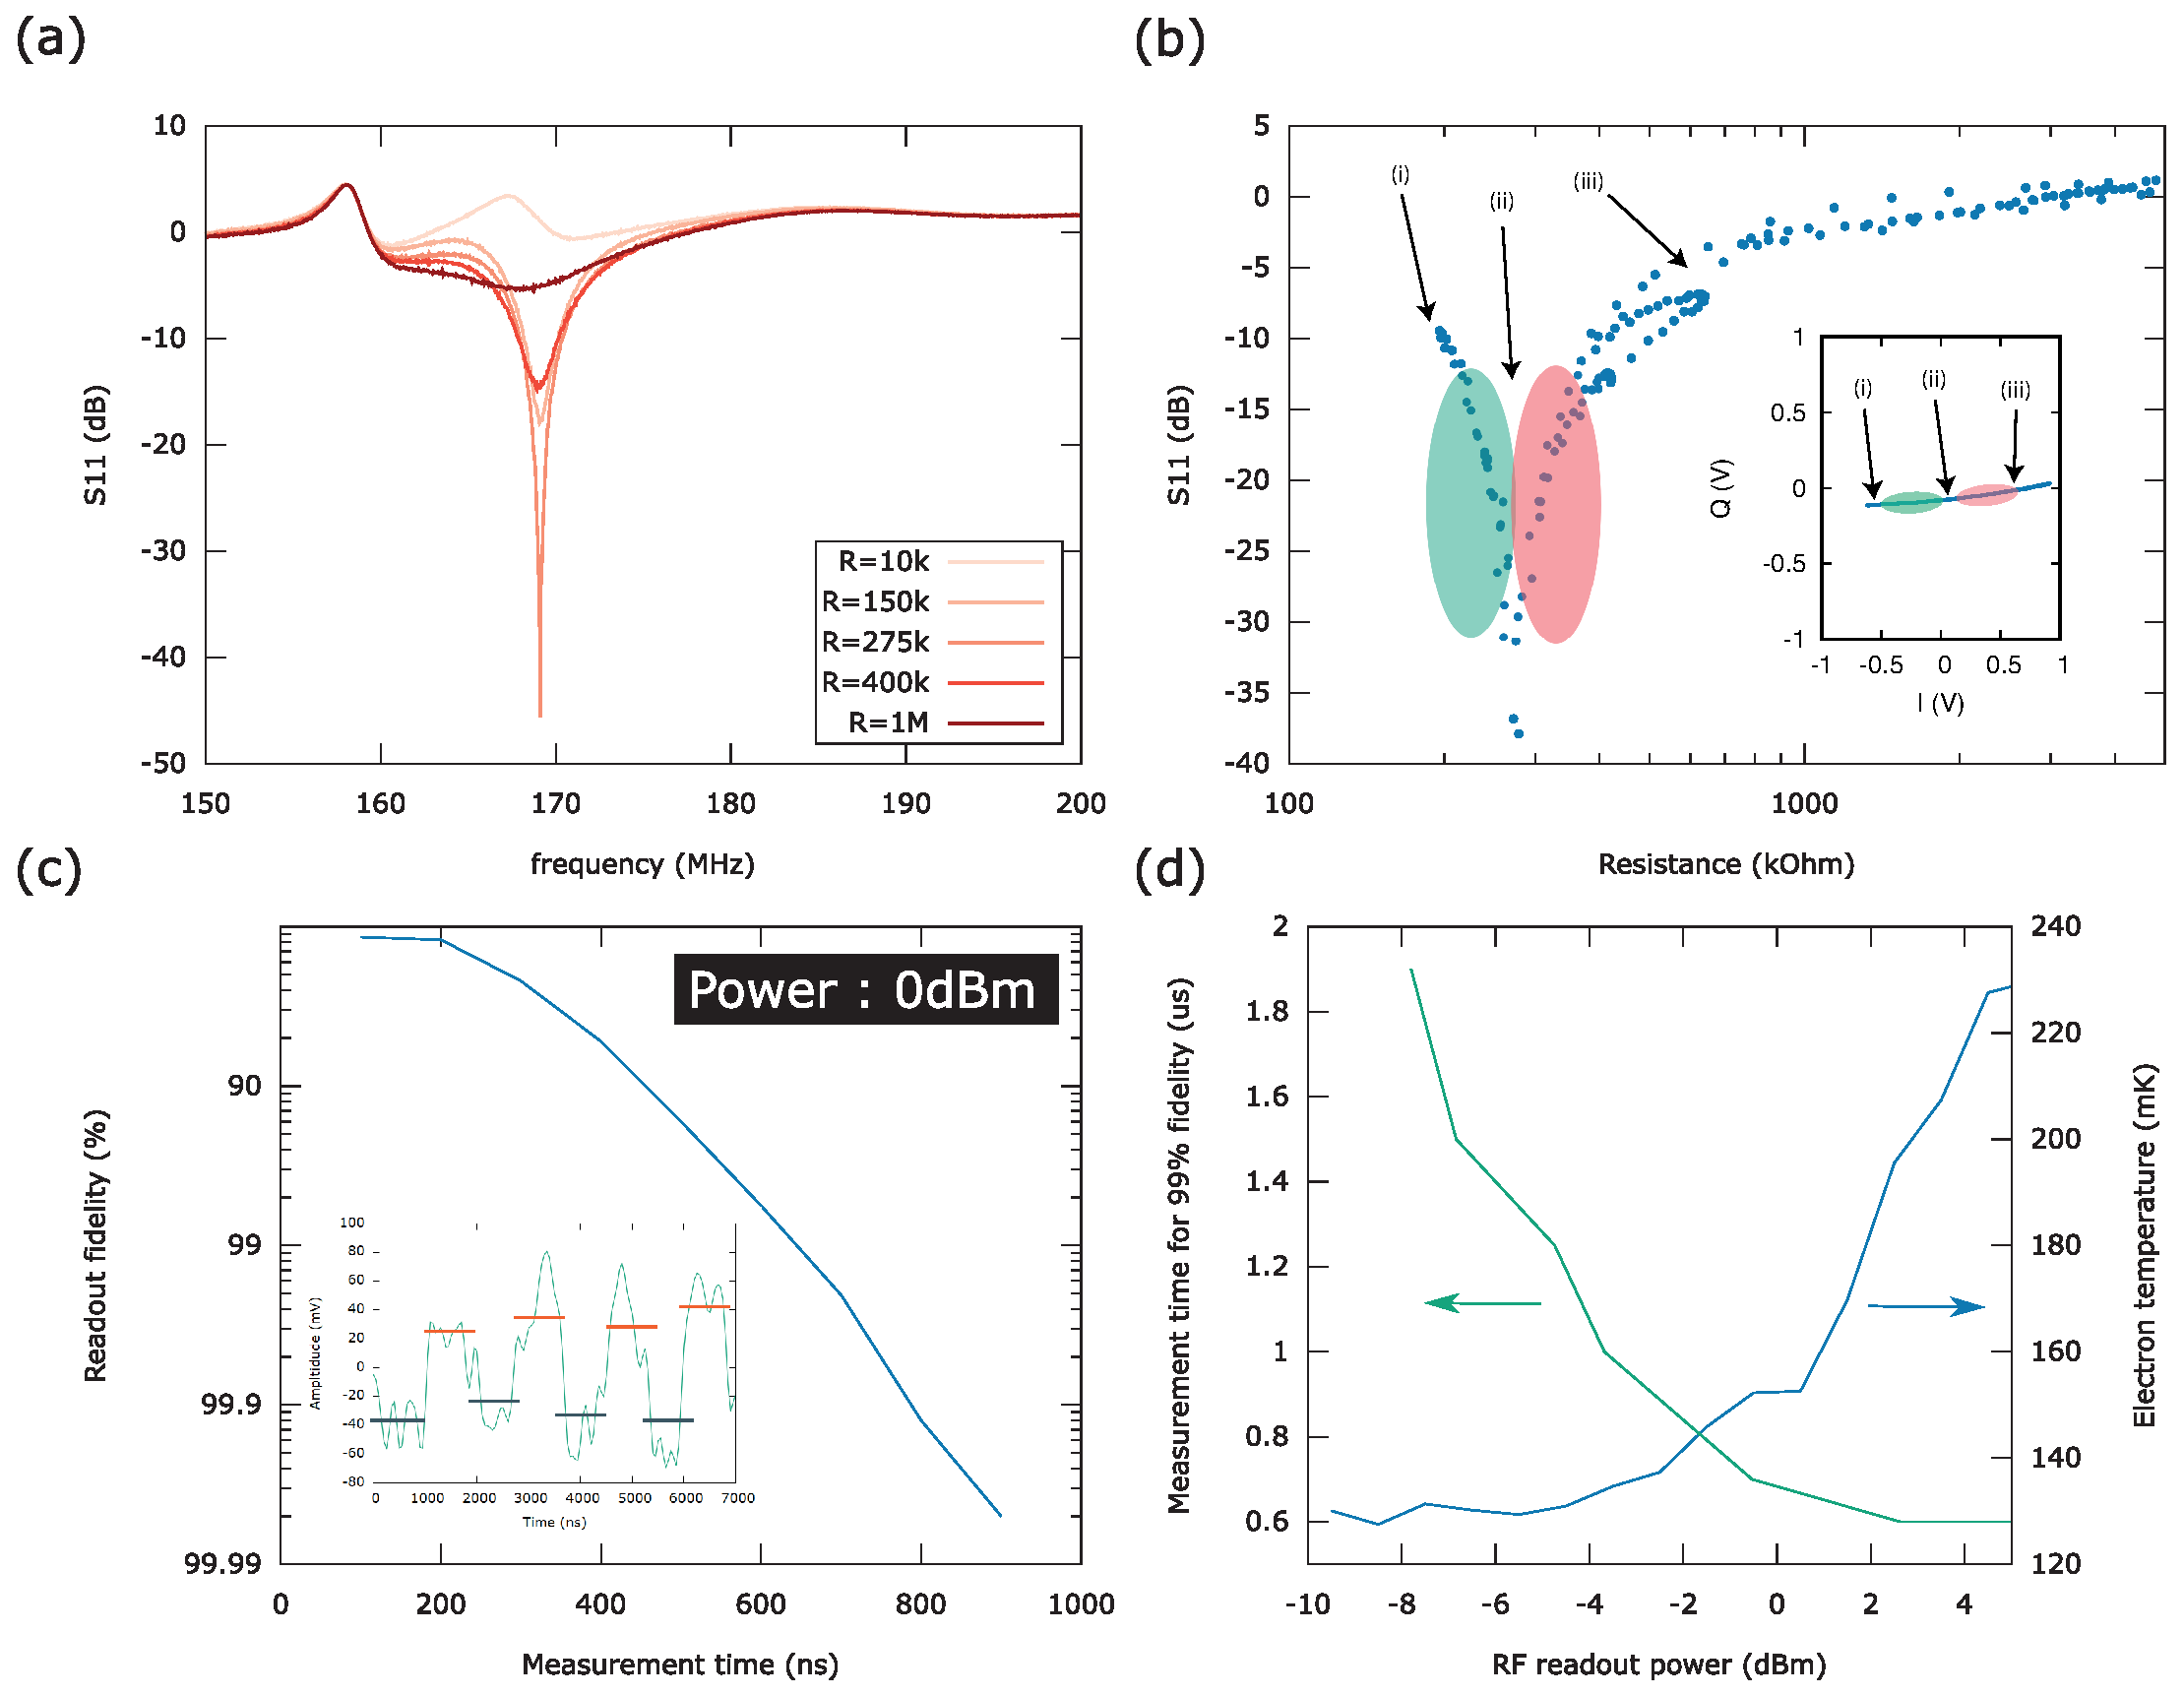
\includegraphics[width=\textwidth]{figures/Performance_figure/perfomance_fig_w_inset.eps}
		\caption{Characteristics and performance of the lead gate approach. (a) Reflection coefficient of the matching circuit as a function of frequency for several resistances of the sensing dot. (b) Reflection of the matching circuit at the resonance versus the resistance of the sensing dot. The matching condition of the circuit is met at 275 k$\Omega$. The sensitive regions are marked in red and green respectively. The inset shows the theoretical reponse for this circuit in the IQ plane. (c) Infidelity of charge detection versus measurement time for a intradot transition. The inset shows an example time trace of the signal. (d) Curves showing the relationship between the charge readout fidelity and the electron temperature versus the applied power to the matching circuit. The electron temperature was determined by measuring the polarization line \cite{van2018automated}. }
		\label{fig:lead_gate_result}
	\end{figure}	

	In figure \ref{fig:lead_gate_result}(a), the response of the resonator versus frequency is shown for several resistances. From this figure, one can derive the bandwidth (FWHM) of the matching circuit, as it is equal to the linewidth of the resonance curve. At $R_{MATCH}$, the expected bandwidth is 0.8 MHz. In other words, we cannot measure signals faster than $\sim$ 600 ns.
	\\ \\
	% comment yinyu, mention frequency, but is it not implicit you want to work at the resonce frequency?
	In figure \ref{fig:lead_gate_result}(b), we characterize the reflectance of the matching circuit versus $R_{SD}$. The matching resistance ($R_{MATCH}$) is 275 k$\Omega$ at the matching frequency. There are two highly sensitive regions around the matching resistance as indicated in figure \ref{fig:lead_gate_result}(b). The inset shows the theoretical phase/amplitude response around $R_{match}$. In most works, the resistances that are measured are larger than $R_{match}$ (from (c) to (b) in the inset).
	From theory, one should be able to achieve the maximal SNR when operating in the range that is indicated by (i) and (iii) in the inset. Point (i) and (iii) is differentiable by their phase ($\Delta \phi = \pi$), as shown in the IQ plane. In other words, we recommend to choose the matching point such that the resistance range you want to measure is covered by both the sensitive regions. \\
	The resistance of our sensing dot is in the range of 400k$\Omega$ to 1M$\Omega$. Our matching resistance is just below these values. This means we are missing out on a factor $\sim2$ of signal to noise ratio. We could reach a matching resistance within this range (e.g. 600k$\Omega$) if we would reduce our parasitic capacitance ($C_p$) from 250 fF to 150 fF (e.g. by making the footprint of the gates smaller).
	\\ \\
	The characterize the performance of the readout, we measured the charge readout fidelity. This fidelity is defined as the probability to correctly determine if a quantum dot is occupied with zero (N=0) or one (N=1) electron for a given measurement time. To calculate the fidelity, we send a train of block pulses (10k) to the quantum dot which will enforce the charge state N=0 or N=1 (top/bottom of the block pulse). We sample for each half period of the block pulse the signal of the sensing dot. This gives a distribution of the signals collected for the occupation N=0 and N=1. The overlap of both signals is the reported fidelity. For these measurements, we used a digital bandpass filter (FIR type) between 100 kHz and 2.5 MHz. The lower frequency of the passband was determined by the slowest signal we wanted to see (e.g. 5 $\mu$s in this case). The upper frequency was taken larger than the bandwidth of the matching circuit to not limit the measurement results.
	\\ \\
	In figure \ref{fig:lead_gate_result}(c), the charge readout fidelity versus the measurement time is plotted. A charge readout fidelity of 99\% can be reached in 700 ns. For these short measurement times, the fidelity us most likely limited by (1) the signal to noise ratio and/or (2) the effective bandwidth of the matching circuit. The SNR is also strongly correlated to the applied power. In figure \ref{fig:lead_gate_result}(d) the readout fidelity and the electron temperature versus the applied power are plotted. We see that there is a clear trade off between applied power, fidelity and electron temperature.  
	When applying high powers ($>0dBm$), the readout fidelity does not improve anymore. In this regime, we are most likely limited by the bandwidth of the matching circuit (0.8 MHz). For lower powers, we are SNR limited, as increasing the power does increase the fidelity. In general one wants to limit the applied power to ensure low electron temperatures of the quantum dots. Therefore we also recommend to only supply power to the RF readout circuit when readout is being done. 

\section{Conclusion}
In this work we demonstrated two methods that can be used to achieve a reasonable matching condition in accumulation mode devices. For the ohmic method, the split gate design was used to generate a tunable contact resistance. We showed that when $R_c$ is increased, the matching resistance will also increase. This allows for in situ tuning of $R_{MATCH}$. One has to be be careful though, as a non-reactive component is introduced in the matching network. This affects the power transfer to the sensing dot hence the SNR of the readout. \\ \\
Using the same split gate design, it is also possible to connect the RF source directly to the accumulation gate of the sensing dot. The split gate method allows for state of the art readout performance. A charge state can be read out within $1\mu s$ with a $>$99.9\% fidelity. This performance is comparable to other recent works \cite{Connors2020,noiri2020radio}. In these works, the capacitance $C_{2DEG}$ is kept small by smart gate design. We consider both the works in \cite{Connors2020,noiri2020radio} and the split gate method equal, as the effective matching circuit in both cases can be reduced to the standard LCR circuit. One scenario where the split gate method would have a clear advantage, is when one has a large contact resistance $R_c$ and/or large 2DEG capacitance, $C_{2DEG}$ is unavoidable. This could for example be the case for quantum dots made in SiMOS.
\\
\\
\section{stuff} % (fold)
\label{sec:stuff}
random stuff\\
move :: ? :: This  suggests that it should possible to remove the ohmic and the lead gate altogether. Note that this could make the tune up of the device harder, as no transport measurements through the sensing dot would be possible.
\\ \\
to be moved / sup?:: 
An image of our inductor and chip is shown in figure\ \ref{fig:overview}(e). The parasitic capacitance ($C_p$)  of the circuit can be broken down in 3 parts: the self-capacitance of the inductor, bond wire from the inductor to the chip and capacitance of the chip. The self-capacitance of the inductor is around 50 fF, this is kept low using high kinetic inductance materials. We estimate the capacitance of the bond wire to be around 50 fF from Comsol simulations. The chip capacitance is estimated to be 150 fF using a microstrip model.

\printbibliography

\end{document}
